
\begin{figure}[ht]
\begin{Verbatim}[numbers=left,fontsize=\codesize,commandchars=\*\{\}]
type left(node, node Child).*label{line:language:dict_header1}*hfill // Predicate declaration
type right(node, node Child).
type linear value(node, int Key, string Value).
type linear replace(node, int Key, string Value).*label{line:language:dict_header2}

replace(A, K, New),*label{line:language:dict_first1}*hfill// Rule 1: we found our key
value(A, K, Old)
   -o value(A, K, New).*label{line:language:dict_first2}

replace(A, RKey, RValue),*label{line:language:dict_second1}*hfill// Rule 2: go left
value(A, Key, Value),
RKey < Key,
!left(A, B)
   -o value(A, Key, Value),
      replace(B, RKey, RValue).*label{line:language:dict_second2}

replace(A, RKey, RValue),*label{line:language:dict_third1}*hfill// Rule 3: go right
value(A, Key, Value),
RKey > Key,
!right(A, B)
   -o value(A, Key, Value),
      replace(B, RKey, RValue). *label{line:language:dict_third2}
\end{Verbatim}
\caption{LM program for replacing a key's value in a BST dictionary.}
\label{code:language:btree_replace}
\end{figure}

Our second example, shown in Fig.~\ref{code:language:btree_replace}, implements
the key update operation for a binary search tree~(BST) represented as a
key/value dictionary. Each LM node represents a binary tree node. We first
declare all the predicates in
lines~\ref{line:language:dict_header1}-\ref{line:language:dict_header2}.
Predicates \code{left} and \code{right} represent the child nodes of each BST
node. Linear predicate \code{value} stores the key/value pair of a node, while
the linear predicate \code{replace} represents an update operation where the key
in the second argument is to be updated to the value in the third argument.

The algorithm uses three rules for the three possible cases of updating a key's
value. The first rule
(lines~\ref{line:language:dict_first1}-\ref{line:language:dict_first2}) performs
the update by removing \code{replace(A, K, New)} and \code{value(A, K, Old)} and
deriving \code{value(A, K, New)}. The second rule
(lines~\ref{line:language:dict_second1}-\ref{line:language:dict_second2})
recursively picks the left branch for the update operation by deleting
\code{replace(A, RKey, RValue)} and re-deriving it at node \code{B}. Similarly,
third rule
(lines~\ref{line:language:dict_third1}-\ref{line:language:dict_third2})
recursively descends the right branch. The derivation of \code{replace} facts on
node \code{B} can also be seen as a implicit \emph{message passing} from
\code{A} to \code{B}, since \code{B} is a different node than \code{A} and the
LHS of each rule can only manipulate facts from the same node.

The initial facts of the program are presented in
Fig.~\ref{code:language:btree_replace_initial} and describe the initial binary
tree configuration, including keys and values, and the \code{replace(@1, 6,
"x")} fact instantiated at the root node \code{@1} that manifests the intent to
change the value of key 6 to "x".

\begin{figure}[ht]
\begin{Verbatim}[numbers=left,fontsize=\codesize,commandchars=\*\{\}]
!left(@1, @2).
!right(@1, @3).
!left(@2, @4).
!right(@2, @5). 
!left(@3, @6).
!right(@3, @7).

value(@1, 3, "a").
value(@2, 1, "b").
value(@3, 5, "c").
value(@4, 0, "d").
value(@5, 2, "e").
value(@6, 4, "f").
value(@7, 6, "g").

// Update key 6 to value "x".
replace(@1, 6, "x").
\end{Verbatim}
\caption{Initial facts for replacing a key's value in a BST dictionary.}
\label{code:language:btree_replace_initial}
\end{figure}

Figure~\ref{fig:language:btree_trace} represents the trace of the algorithm. The program
database is partitioned by the seven nodes using the first argument of each
fact. In Fig.~\ref{fig:language:btree_trace}~(a), we present the database filled with the
program's initial facts. Next, we follow the right branch using rule 3 since $6
> 3$ (Fig.~\ref{fig:language:btree_trace}~(b)).  We use the same rule again in
Fig.~\ref{fig:language:btree_trace}~(c) where we finally reach the key 6. Here, we apply
rule 1 and \code{value(@7, 6, "g")} is updated to \code{value(@7, 6, "x")}.

\begin{figure}[h]
        \centering
        \begin{subfigure}[b]{0.5\textwidth}
                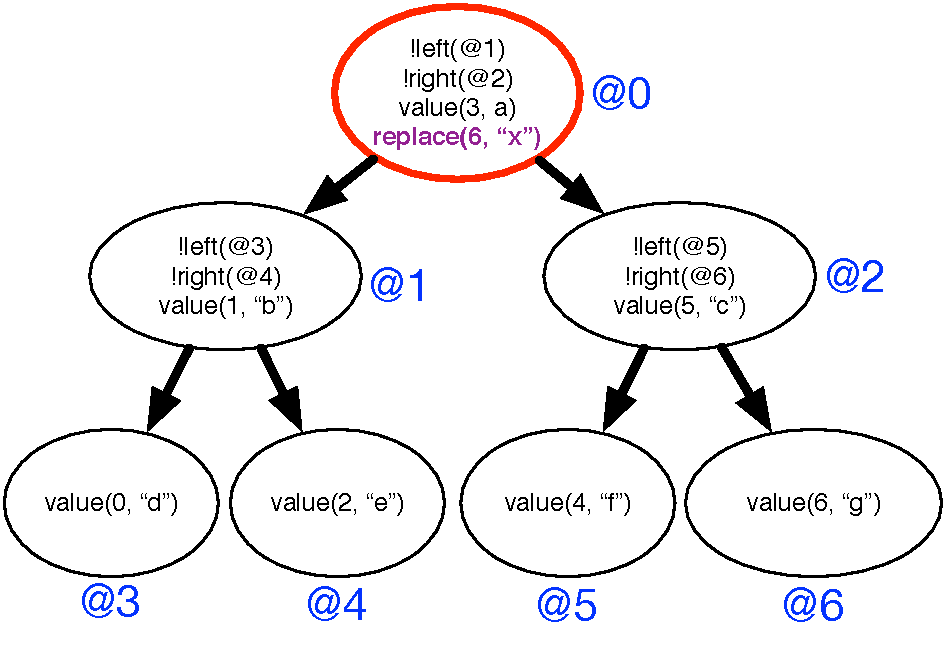
\includegraphics[width=\textwidth]{figures/btree/btree_trace1}
                \caption{Initial database.}
                \label{fig:language:btree_trace1}
        \end{subfigure}%
        ~
        \begin{subfigure}[b]{0.5\textwidth}
                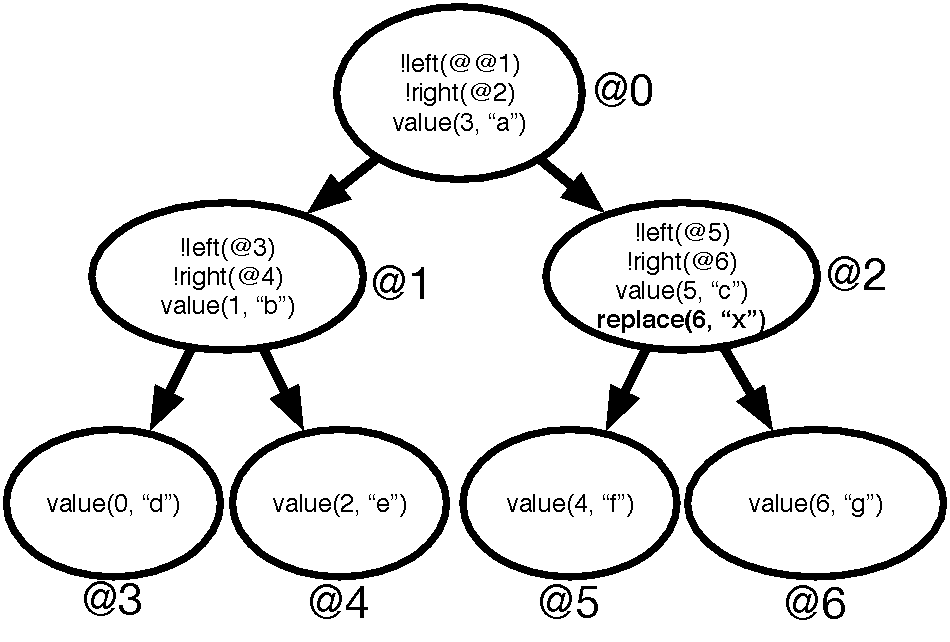
\includegraphics[width=\textwidth]{figures/btree/btree_trace2}

                \caption{After applying rule 3 at node \code{@1}.}

                \label{fig:language:btree_trace2}
        \end{subfigure}\\
        \begin{subfigure}[b]{0.5\textwidth}
                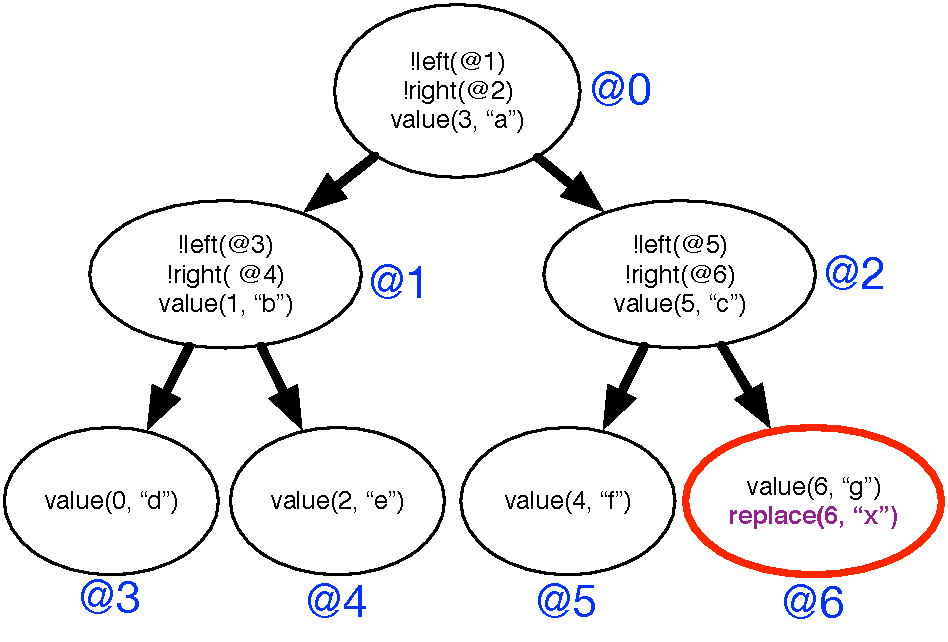
\includegraphics[width=\textwidth]{figures/btree/btree_trace3}
                \caption{After applying rule 3 at node \code{@3}.}
                \label{fig:language:btree_trace3}
        \end{subfigure}%
        ~
        \begin{subfigure}[b]{0.5\textwidth}
                  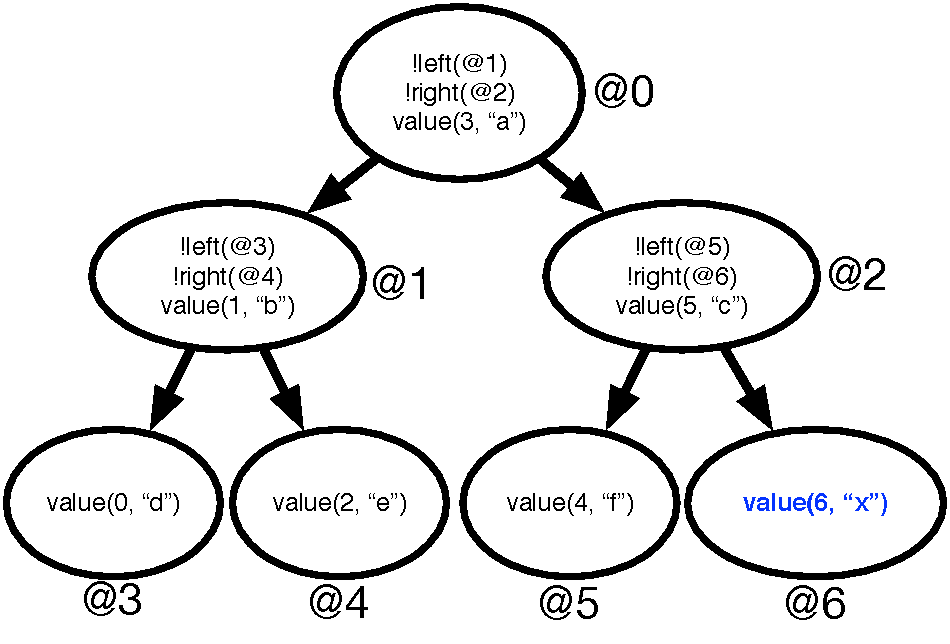
\includegraphics[width=\textwidth]{figures/btree/btree_trace4}
                  \caption{After applying rule 1 at node \code{@7}.}
                  \label{fig:language:btree_trace4}
          \end{subfigure}
        \caption{An execution trace for the binary tree dictionary
           algorithm. The first argument of each fact was dropped and the
           address of the node was placed beside it.}\label{fig:language:btree_trace}
\end{figure}

Like the message routing example shown in the previous section, the amount of
concurrency present in this example depends on the number of \code{replace}
facts. If there are many \code{replace} operations to perform on different parts
of the BST, then there is more concurrency. On the other hand, if only a few BST
nodes are being updated, then concurrency is reduced. This is the same behavior
that one would expect from an parallel implementation of the BST data structure
in an imperative language.
